\chapter{Neuro-Fuzzy-Systeme}

Im vorletzten Kapitel wurden zwei Arten von Fuzzy-Systeme, oder Reglern, vorgestellt. Solche Systeme werden in der Praxis öfters mit Konzepte aus der Künstliche Intelligenz kombiniert. Zum einen bietet sich Kombinationen mit Neural Networks \ref{ANN}, Evolutionäralgorithmen und vielen weiteren. Im folgenden Kapitel wird besonders die Kombination mit Neuronalen Netzen untersucht. Die Zusammenarbeit von Fuzzy-Reglern und Neuronalen Netzen ist atraktiv, weil die Interpretierbarkeit von Fuzzy-Systeme mit den Lernmöglichkeit von Neuronalen Netzen effektiv zu verbinden ist. In den nächsten Unterkapiteln werden zwei Arten von Modelle mit jeweils einer Beispielstruktur - Modelle für feste Lernaufgaben und solche mit verstärkendem Lernen. Die Modelle werden außerdem in der Literatur als Neuro-Fuzzy-Systeme, bzw. Neuro-Fuzzy-Regler, bezeichnet. \cite{CIKruse:15}
\section{Neuro-Fuzzy-Regler}

Neuro-Fuzzy-Regler, oder Neuro-Fuzzy-Systeme, sind Modelle, bei denen konzeptionelle Teile von Neuronalen Netzen und Fuzzy-Systeme kombiniert werden. Das Ziel dieser Reglern ist es das beste aus beiden Welten zu kombinieren - Lernbarkeit von Neuronalen Netzen und Interpretierbarkeit von Fuzzy-Systeme. Außerdem bietet Fuzzy-Systeme die Möglichkeit Vorwissen einzubrigen, was hingegen die Lernzeit der Neuronalen Netze verkürzt. Am Ende des Lernprozesses erhält man ein Modell, dessen Regelungsstragie interpretierbar ist und dessen Regelung überprüft und eventuell noch angepasst werden können \cite{CIKruse:15}. Demnächst werden zwei Arten von Neuro-Fuzzy-Modelle, die unterschiedliche Anwendungsfälle haben.

\subsection{Modell f\"{u}r feste Lernaufgaben}
%(Muss Änderungen unterliegen)

Neuro-Fuzzy-Modell für feste Lernaufgaben versuchen, Fuzzy-Mengen und, bei TSK-Modelln, die Parameter der Ausgabefunktion unter Einreichung einer Mengen von Ein-/Ausgabe-Tupeln zu optimieren. Diese Modell sind genau dann sinnvoll, wenn schon eine Fuzzy-Regelbasis vorliegt. Die Regelbasis unterliegt infolge des Lernens eine Verarbeitung, die als Ziel eine Optimierung hat. %Dafür sind geieignete Ein-/Ausgabedaten gebraucht.

Ein weiteres Anwendungsbeispiel ist bei bereits existierender Regelbasis, dass dieser mit einer neuen ausgetauscht wird. Falls die Basis schon errechnete Werte geliefert hat, können diese zusammen mit den zugehörigen Eingabewerten dem Neuro-Fuzzy-System zum Lernen gegeben werden. Am Ende erhält man eine optimierte Fuzzy-Regel-Basis, die die alte Basis ``ersetzt''.

Falls es keine angemessene Lernaufgabe bereits gegeben ist, dann eignet sich dieses Verfahren nicht. Es existieren natürlich Ansätze, die es ermöglichen, einen initialen Regelbasis aus Eingabedaten zu erstellen. Ein solcher Verfahren wird später noch vorgestellt.

Folglich wird ein Beispiel von einem Modell, das sich für feste Lernaufgaben eignet, vorgestellt. Es geht nämlich um das ANFIS-Modell.

\subsubsection{Das ANFIS-Modell}

Im Frühjahr von 1993 wurde das Neuro-Fuzzy-System ANFIS (Adaptive Neuro-Fuzzy Inference System oder Adaptive Network-based Fuzzy Inference System) entwickelt. Das Modell wurde in mehrere Software-Pakete schon eingesetzt. Die ANFIS basiert auf einer hybriden Struktur, sodass es sowohl als ein Neuronales Netz, als auch als ein Fuzzy-System interpretiert werden kann. In dem System sind Regeln angelegt, die nach dem TSK-Modell definiert sind (Takagi-Sugeno-Kang-Reglern \ref{TSK}). Die Abbildung \ref{ANFIS_Abb} zeigt einen Modell mit folgender Regelbasis:(%Abbildung hier zitieren aus Buch 2)

\begin{center}
	$R_1$: Falls $x_1$ ist $A_1$ und $x_2$ ist $B_1$, dann ist $y$=$f_1$($x_1$,$x_2$)\\
	
	$R_2$: Falls $x_1$ ist $A_1$ und $x_2$ ist $B_2$, dann ist $y$=$f_2$($x_1$,$x_2$)\\
	
	$R_3$: Falls $x_1$ ist $A_2$ und $x_2$ ist $B_2$, dann ist $y$=$f_3$($x_1$,$x_2$)\\
\end{center}

Dabei sind $A_1$, $A_2$, $B_1$ und $B_2$ linguistische Termen, die den entsprechenden Fuzzy-Mengen $\mu_i^{(j)}$ zugeordnet sind. Die Funktionen $f_i$ sind linear und sehen wie folgt aus (siehe \ref{FDF}):
\begin{equation}
	f_i(x_1, x_2) = p_0^{i} + p_1^{i}\cdot x_1 + p_2^{i}\cdot x_2
\end{equation}

Der Konklusionsfunktion $f_i$ entspricht die Regel $R_i$. Somit hat jede Regel eine eindeutige Ausgangsfunktionen mit eindeutigen Parametern $p_0^{i}, p_1^{i}, p_2^{i}$.

Die Ausgabe eines ANFIS-Modells berechnet sich genau so wie ein TSK-Modell (siehe \ref{FDF}). %Zuerst wird der Zugehörigkeitsgrad einer Regel mit dem entsprechenden Konklusionsfunktion multipliziert. WeiterhinAnschließend normiert man das Resultat  summiert man das Resultat aus allen Regeln und teilt die Summe durch die Summe aller Anktivierungsgraden. 
Für den genannten Beispiel lautet die Ausgabe:
\begin{align}
	f = \dfrac{\sum_{i}^{3} \tilde{w_i}\cdot f_i(x_1, x_2)}{\sum_{i}^{3} \tilde{w_i}}
\end{align}

Der ANFIS-Ansatz besteht aus 5 Schichten. Die Abbildung \ref{ANFIS_Abb} veranschaulicht die Struktur.

\begin{figure}[htbp]
	\centering
	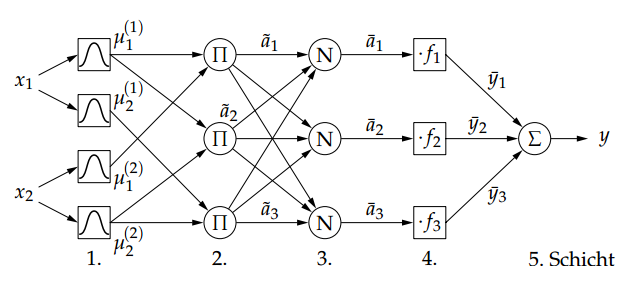
\includegraphics[scale=0.5]{images/ANFIS_Abb.png}
	\caption{ANFIS-Model \cite{CIKruse:15}}\label{ANFIS_Abb}
\end{figure}

In der \textbf{ersten Schicht} werden die Eingabewerte eingereicht und entsprechend die Zugehörigkeiten zu den Fuzzy-Sets ausgegeben. Weiterhin werden in der \textbf{zweiten Schicht} die Aktivierungswerte jeder Regel ausgewertet. Die Neuronen werden mit $\prod$ gekennzeichnet. Einzelnen Fuzzyzugehörigkeitswerte werden mittels Operatoren kombiniert, um die Aktivierungsgrad jeder Regel zu berechnen. Hier dürfen Operatoren zur Verknüpfung von Fuzzy-Mengen eingesetzt werden, üblicherweise der UND-Operator (siehe \ref{AND}). Die Gleichung \ref{eq3_3} ergibt die Berechnung bei gegebener UND-Verknüpfung:

\begin{equation}\label{eq3_3}
	\tilde{w}_i = \prod \mu_i^j(x_j)
\end{equation}

Die Variable $\tilde{w}_i$ ergibt die Aktivierung, oder Erf\"{u}llungsgrad, des Regels $R_i$ und $\mu_i^j$ ist die $j.$ Zugehörigkeitsfunktion in der Regel $R_i$.

Im \textbf{dritten Schicht} findet die Normalisierung aller Aktivierungswerte $\tilde{w}_i$ statt. Mit einfachen Worten wird der Beitrag berechnet, den jeder Regel für den Gesamtausgabe beiträgt. Nach der Normalisierung erhält man Aktivierungsgrößen zwischen $0$ und $1$. Die Gleichung \ref{barwi} berechnet die normalisierten Werten für jeden Regel $R_i$:

\begin{equation}\label{barwi}
\bar{w}_i = \frac{\tilde{w}_i }{\sum_j \tilde{w}_j } 
\end{equation}

Im \textbf{vierten Schicht} berechnen die mit $N$ markierten Neuronen die gewichteten Ausgabewerte. Das ``Gewicht'' (Ergebnis) aus dem letzten Layer wird mit der entsprechenden Ausgabefunktion multipliziert:

\begin{equation}
\bar{y}_i = net_i = \bar{w}_i\cdot f_i(x_1, ..., x_n). 
\end{equation}

Im \textbf{fünften Schicht} steht ein einziges Neuron, der mit $\sum$ beschriftet ist. Im letzten Schicht berechet man die Ausgabe, indem alle Werte aus dem \textbf{vierten Schicht} zusammenaddiert werden:

\begin{equation}
y = y_{out} = \sum_i \bar{y}_i = \frac{\tilde{w}_i\cdot f_i(x_1, ..., x_n)}{\sum_j \tilde{w}_j}.
\end{equation}

Diese Struktur ähnelt sich der von TSK-Modell. Für die Optimierung von Parametern der Zugehörigkeitsfunktionen und Konklusionsfunktionen eignet sich der ANFIS-Ansatz.

Das ANFIS-Modell ermöglicht die Optimierung von Modellparametern - die Fuzzy-Mengen- und Ausgabefunktionsparametern. Diese können erlernt werden, wenn eine angemessene Lernaufgabe vorliegt. Außerdem muss eine ausreichende Menge von Ein-/Ausgabe-Werten zur Verfügung stehen. Es bieten sich mehrere Lernmethoden zur Optimierung der Parametern. Zwei davon sind Gradientenverfahren(analog zur Fehler-Rückpropagation-Verfahren aus Neuronalen Netzen) und die Kleinste-Quadrate-Methode. \cite{CIKruse:15} \cite{Jang:93}

\subsection{Modell mit verstärkendem Lernen}

Bei Modellen mit verstärkendem Lernen wird versucht, die Menge der Daten für das Lernen möglichst gering zu halten. Der Unterschied zwischen Modell mit verstärkendem Lernen und solchen für feste Lernaufgaben besteht darin, dass bei dem Erstgenannten keine Vorwissen bekannt werden müssen, was öfters der Fall sein kann. Es reicht nur, wenn im Laufe des Lernens angegeben wird, ob die Richtung der Optimierung sinnvoll ist.

Ein großes Problem beim verstärkendem Lernen besteht darin, vorzusagen, wie groß der Einfluss einer Regelaktion auf das Gesamtsystem ist. Dieses Problem wird als \textit{Credit Assignment Problem} bezeichnet.

Es existiert eine große Mengen von Modelln mit verstärkendem Lernen, alle aber basieren auf dem gleichen Prinzip. Das System wird zwei Teilsysteme aufgeteilt: zum einen der ``Kritiker''(das ``kritisierende'' System) und der Aktor(zuständig für die Anwendung und Abspeicherung der Regelungsstrategie). Der Kritiker ``äußert'' seine Meinung über den jetzigen Zustand unter Berücksichtigung der vorhergehenden Zustände und somit entscheidet der Aktor anhand der Bewertung, ob eine Korrektur der Regelbasis gemacht werden soll. \cite{CIKruse:15}  \cite{UNIMAG:97}

\subsubsection{Das NEFCON-Modell}

Ziel des NEFCON-Modell, Neuro-Fuzzy Control Modell, ist es, eine interpretierbare Fuzzy-Regelbasis mit möglichst kleinen Trainingsschritten zu erlernen. Das Modell unterscheidet sich von dem ANFIS, indem es erlaubt einen Regelbasis, ohne Vorwissen zu erlernen. Dieses Modell bietet natürlich auch die Möglichkeit, Vorwissen mitzubringen. Das heißt sowohl Fuzzy-Systeme mit vorhandenen Regelbasis, als auch solche mit unvollständiger Fuzzy-Regelbasis. Alle diese Vorteilen sprechen für das NEFCON gegenüber andere Modelle.

Das NEFCON-Modell basiert auf ein Mamdani-Regler. Zum Veranschaulichung wird hier einen kleinen Beispiel mit Grafik \ref{NEFCON_Abb} und Regelbasis gegeben. \cite{CIKruse:15}

\begin{figure}[htbp]
	\centering
	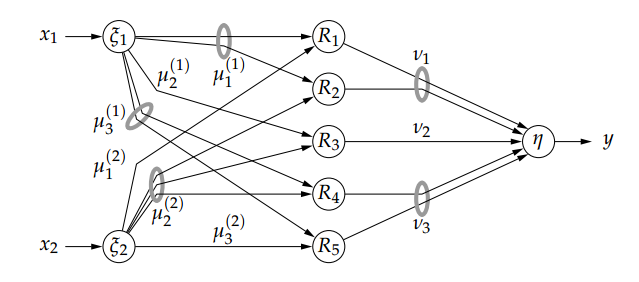
\includegraphics[scale=0.5]{images/nefcon_abb.png}
	\caption{NEFCON-Modell \cite{CIKruse:15}}\label{NEFCON_Abb}
\end{figure}

\begin{center}\label{nef_regelbasis}
	$R_1$: IF $x_1$ in $A_1^{(1)}$ AND $x_2$ in $A_1^{(2)}$, THEN y is $B_1$ \\
	$R_2$: IF $x_1$ in $A_1^{(1)}$ AND $x_2$ in $A_2^{(2)}$, THEN y is $B_1$ \\
	
	$R_3$: IF $x_1$ in $A_2^{(1)}$ AND $x_2$ in $A_2^{(2)}$, THEN y is $B_2$\\
	
	$R_4$: IF $x_1$ in $A_3^{(1)}$ AND $x_2$ in $A_2^{(2)}$, THEN y is $B_3$\\
	
	$R_4$: IF $x_1$ in $A_3^{(1)}$ AND $x_2$ in $A_3^{(2)}$, THEN y is $B_3$
\end{center} 

% Hier Grafik einfügen

Das NEFCON-Modell basiert auf einem generischen Fuzzy-Perzeptron. Das Modell konnte in drei Schichten aufgeteilt werden. Die \textit{erste Schicht} besteht natürlich aus den Eingangsneuronen. Die ist eindeutig und will nicht weiter darauf eingehen. In der \textit{zweiten Schicht} befinden sich die inneren Neuronen, die die Regeln einer Fuzzy-System widerspiegeln. Im Beispiel sind insgesamt fünf Regeln gegeben. Die Fuzzy-Mengen $\mu_r^{(i)}$, die in Mehrere Regeln vorhanden sind, werden durch Ellipse zusammengeführt. Falls beim Lernen eine Anpassung an einem Gewicht durchgeführt werden soll, muss dies in allen Verbindungen gemacht werden, wo die Menge figuriert.

Der eigentliche Lernprozess besteht aus zwei Phasen. In der erste Phase wird versucht, eine Regelbasis erlernt zu werden. Diese Phase wurde weggelassen, falls schon eine existiert. Es lassen sich auch unvollständige sogar fehlende Regelbasen lernen. Für das Letztere ist ein weiterer Algorithmus erforderlich.

In der zweiten Phase findet die Optimierung statt. Dabei werden Fuzzy-Sets modifiziert oder selbst die Verbindungen zu den Regeln umgetauscht. In dem NEFCON-Modell wird als Bewertungsmaß, der ``Kritiker'', ein Fuzzy-Error verwendet. Damit die Optimierung optimal ausgeführt werden kann, sollte das Vorzeichen des Ausgabewertes bekannt sein. Darüber hinaus wird ein erweiterter Fuzzy-Error $E^*$ berechnet:
	\begin{equation}\label{EFE}
	E^* = sgn(y_{out})\cdot E(x_1, \ \ldots , \ x_n)
	\end{equation}
\cite{CIKruse:15} \cite{UNIMAG:97}
\subsubsection{Erlernen einer Regelbasis}

Es existieren mehrere Algorithmen zum Erlernen von Regelbasis. Die Methoden können in drei Kategorien aufgeteilt werden: solche, die ohne vordefinierte Regelbasis startet; solche mit vollständiger Regelbasis und solche mit zufälliger Basis  starten. In den folgenden zwei Unterkapiteln werden Methode für die ersten zwei Kategorien vorgestellt. Bei den Methoden wird keine feste Lernaufgabe benötigt. Tatsächlich geht es darum, dass eine Initialbasis aufgebaut wird, ohne eine große Datenmenge mit optimalen Werten bekannt zu sein. \cite{CIKruse:15} \cite{UNIMAG:97}% Bis Hier drübergeguckt

\subsubsection{Top-Down- oder Reduktionsmethode zum Erlernen einer Regelbasis}

Zum Einen wird die Methode der Top-Down-Methode (in der Literatur auch als NEFCON I bekannt) genannt. Das Verfahren erfordt, dass eine vollständige Regelbasis vorhanden ist. Die Regelbasis beinhaltet auch widersprüchliche Regeln, die in Laufe des Prozesses ausgefiltert werden.

Der Prozess kann in zwei Phasen aufgeteilt werden. In der ersten Phase werden alle die Regeln eliminiert, die bei ihrer Ausgabe den falschen Vorzeichen aufweisen. Die auszufilternden Regeln werden mit der erweiterten Fuzzy-Fehler-Funktion (siehe \ref{EFE}) bestimmt. In der zweiten Phase werden Regeln mit identischer Prämisse zufällig ausgewählt. Folglich wird der Fehler für die bestimmte Regel berechnet. Zum Schluss wird die Regel ausgewählt, die die kleinste Fehlerrate aufweist. Die restlichen Regeln werden verworfen.

Eins der Nachteile der Top-Down-Methode ist die Aufwändigkeit, weil es mit einer großen Regelbasis gestartet wird. Das nächste Verfahren ist das Gegenteil von Top-Down-Methode, zwar Bottom-Up-Methode. \cite{CIKruse:15}


\subsubsection{Bottom-Up- oder Eliminationsmethode zum Erlernen einer Regelbasis}

Der Bottom-Up-Algorithmus beginnt mit einer leeren Regelbasis. Jedoch muss eine initiale Aufteilung(Intervall) der Ein- und Ausgabewerten gegeben sein. Analog zur Top-Down besteht diese Methode auch aus zwei Phasen. 

Erste Phase beginnt mit der Bestimmung der Prämisse für die Regeln. Der Prozess evaluiert jede Fuzzy-Menge mit bestimmten Eingaben und die Mengen, die den höchsten Zugehörigkeitsgrad aufweisen, werden ausgewählt. Aus den ausgewählten Fuzzy-Mengen werden neue Regeln gebaut. Danach versucht der Algorithmus eine geeignete Ausgabe aus dem aktuellen Fuzzy-Fehler zu ``raten''. Dabei wird vorausgesetzt, dass Eingaben mit ähnlichen Fehlerwerten ähnliche Ausgaben liefern.

In der zweiten Phase werden die Fuzzy-Mengen in den Konklusionen optimiert. Dabei werden nicht die Parametern der Konklusionen angepasst, sondern bei Bedarf die Fuzzy-Menge durch eine andere ersetzt.

Wegen des inkrementellen Lernen lässt sich einfach Vorwissen in dem Regelbasis einführen. Bei den Fällen mit unvollständigen Regelbasen werden passende Regeln hinzugefügt. Das Verfahren garantiert jedoch nicht, dass immer eine geeignete Regelbasis aufgebaut wird. Aus diesem Grund ist es empfohlen, dass die Regelbasis manuell am Ende des Lernens überprüft und entsprechend angepasst wird. \cite{CIKruse:15} \cite{UNIMAG:97}

\subsubsection{Optimierung der Regelbasis}

Die Optimierung bei NEFCON verwendet die Methode ``Back Propagtion Method'', oder Rückpropagationsmethode. Der Fehler wird rückwirkend durch das Netz geführt und lokal bei jeder Fuzzy-Menge angewendet.

Eine Änderung darf sowohl in den Prämissen, als auch in den Konklusionen. Es wird das Prinzip des verstärkenden Lernens angewendet. Das bedeutet, dass für jede Änderung eine Fuzzy-Menge entweder ``bestraft'' oder ``belohnt'' wird. Bestrafung und Belohnung werde in Änderungen wie Verschiebung, Vergrößerung oder Verkleinerung des Bereichs einer Fuzzy-Menge ausgedrückt. Änderungen werden entsprechend iterativ in Beziehung zum Fuzzy-Fehler gemacht. \cite{CIKruse:15} \cite{UNIMAG:97}

\subsubsection{Schlussworte}

% Zusammenfassung der zwei Methoden,
Die Methoden unterscheiden sich in ihrem Kern kaum. Beide Architekturen besitzen entsprechend Vorteile und Nachteile. Der größte Unterschied liegt in der Ausbau ihrer Struktur. ANFIS basiert auf TSK-Modellen, währen NEFCON auf die Mamdani-Reglern. Beide Modelle bieten sie sich gut für das Lernen von Fuzzy-Systeme, jedoch entspricht nur das ANFIS meinem Anwendungsfall - Optimierung von TSK-Modelle.